\documentclass[12pt,a4paper]{article}
\usepackage{graphicx}
\usepackage{mathtools}
\usepackage[utf8]{inputenc}
\usepackage{amsmath}
\usepackage{amsfonts}
\usepackage{amssymb}
\usepackage{amsthm}
\usepackage{float}
\usepackage[left=2cm,right=2cm,top=3cm,bottom=3cm]{geometry}
\usepackage{subfig}
\usepackage{fancyhdr}
\usepackage{multicol}


\newtheorem{theorem}{Teorema}

\renewcommand{\contentsname}{Contenido}
\renewcommand{\refname}{Bibliografía}

\begin{document}

\begin{titlepage}

\begin{center}
	\begin{large}
		TALLER DE RAYOS X
	\end{large}
	
	\vspace{0.2cm}
	
	\textit{Y. Ariza Florez, C. Mendoza Maldonado, J. Rúa Muñoz}\\ 
	Universidad del Atlántico\\
	25 de Marzo de 2020
\end{center}	
\end{titlepage}


	\vspace{0.5cm}
	\newpage
	
	\tableofcontents
	
	\newpage
\section{¿Qué es una red de Bravais?}
\vspace{0.2cm}

Las redes de Bravais son una disposición infinita de puntos discretos cuya estructura es invariante bajo cierto grupo de traslaciones. Las Redes de Bravais o celdas unitarias, son paralelepípedos que constituyen la menor subdivisión de una red cristalina que conserva las características generales de toda la retícula, de modo que por simple traslación del mismo, puede reconstruirse el sólido cristalino completo.[1]\\


\noindent Estas propiedades hacen que desde todos los nodos de una red de Bravais se tenga la misma perspectiva de la red. Se dice que los puntos de una red de Bravais son equivalentes. Se ha demostrado que sólo existe una única red de Bravais
unidimensional, 5 redes bidimensionales y 14 modelos distintos de redes
tridimensionales.\\

\subsection{Elementos de simetría}

\vspace{0.2cm}
\noindent Estos 14 modelos se pueden agrupar en siete sistemas cristalinos, cada uno de los cuales tiene en común ciertos elementos de simetría característicos. Los elementos de simetría que se han escogido para especificar estos siete sistemas son los siguientes:
\vspace{0.2cm}

\begin{itemize}
	
	\item \textit{Eje de rotación de orden n:} La rotación alrededor de un eje de este tipo a un ángulo de $2\pi / n$ radianes no produce ningún cambio en la estructura reticular. En este caso, n puede tener los valores 1, 2, 3, 4 y 6. La simetría rotacional de 5 veces en una red cristalina es imposible.[2]
	
	\vspace{0.2cm}
	
	\item \textit{Plano de simetría:} Una mitad del cristal reflejada en un plano semejante que pasa por un punto de la red, reproduce la otra mitad.
	
	\vspace{0.2cm}
	
	\item \textit{Centro de inversión:}   un punto de la red alrededor del cual la operación $r\longrightarrow - r$ (en donde $r$ es un vector a cualquier otro punto de la red) deja a la estructura reticular sin sufrir cambio alguno.
	
	\vspace{0.2cm}
	
	\item \textit{Eje de rotación-inversión:} la rotación alrededor de este eje a 2n/n radianes (n = 1, 2, 3, 4, 6) seguida de una inversión alrededor de un punto de la red
	por el que pasa el eje de rotación, no produce ningún cambio en la red.
\end{itemize}

\newpage


 \begin{center}
	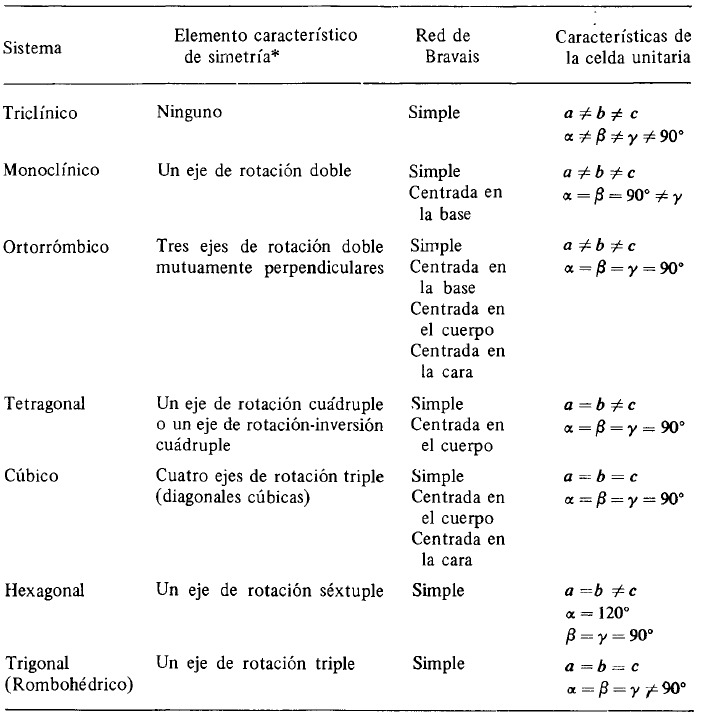
\includegraphics[width=0.85\linewidth]{F1}
\end{center}
\begin{center}
	Tabla 1: Los siete modelos cristalino [2]
\end{center}

\vspace{0.2cm}

\section{¿Qué es una red recíproca?}

La red recíproca es un concepto usado en física y matemáticas para denotar a la transformada de Fourier de una red en el espacio real. Los nodos o puntos que conforman la red recíproca están constituidos por todas las combinaciones lineales de una base vectorial en el espacio recíproco, también conocido en diversas aplicaciones como espacio de Fourier, espacio de momentos o espacio de fases.

El espacio recíproco relaciona variables conjugadas y es un concepto fundamental para el análisis de procesos físicos en los que se produce una transferencia de momento. En cristalografía, los puntos de la red recíproca de la red de Bravais corresponden a las direcciones en las que se puede observar difracción por un cristal.\\


Consideremos los puntos $R_{i}$ que pertenecen a una red de Bravais y una onda plana $e^{i \overrightarrow{K}.\overrightarrow{R}}$. El vector de onda $\overrightarrow{K}$ indica la dirección de propagación y su módulo está relacionado con la longitud de onda  $ \overrightarrow{K} = \frac{2\pi}{ \lamda}$. Para un $\overrightarrow{K}$ cualquiera esta onda no tendrá, en general, la periodicidad de la red $R_{i}$, pero podemos esperar algún fenómeno físico particular en caso que la tenga, esto es:

\begin{equation*}
    f(\overrightarrow{r}) = f(\overrightarrow{r} + \overrightarrow{R_{i}}) \hspace{0.5 cm} Para\hspace{0.2 cm} todo \hspace{0.2 cm} \overrightarrow{r} y \overrightarrow{R_{i}}
\end{equation*}

si 
\begin{equation*}
    f(\overrightarrow{r}) = e^{i \overrightarrow{K_{j}}. \overrightarrow{r}}
\end{equation*}

\begin{equation*}
    e^{i \overrightarrow{K_{j}}.\overrightarrow{r}} = e^{\overrightarrow{K_{j}}. (\overrightarrow{r}+ R_{i})}
\end{equation*}




Para una red unidimensional : $ K_{n}a = 2\pi n = 2\pi \frac{a}{\lamda_{n}}$ \longrightarrow $\lamda_{n} = \frac{a}{n}$

Los vectores de onda $K_{n}$ son tales que entra un número entero de longitudes de onda en a. Cada red de bravais tiene una red reciproca correspondiente. \\

si $\overrightarrow{a_{1}}$ , $\overrightarrow{a_{2}}$, $\overrightarrow{a_{3}}$ son vectores de la celda primitiva, los vectores $\overrightarrow{b_{1}}$, $\overrightarrow{b_{2}}$, $\overrightarrow{b_{3}}$ se pueden generar de la siguiente forma:

\begin{equation*}
    \overrightarrow{b_{i}} =2 \pi \frac{ \overrightarrow{a_{j}}X \overrightarrow{a_{k}}}{ \overrightarrow{a_{1}}. \overrightarrow{a_{2}} X \overrightarrow{a_{3}}}
\end{equation*}

 donde  i, j y k guardan un orden ciclico
 
 \begin{equation*}
     \overrightarrow{b_{k}} . \overrightarrow{a_{l}} = 2\pi \delta_{kl}
 \end{equation*}
 
 Para cualquier vector de las redes directa y reciproca 


\begin{align*}
    \overrightarrow{R} = m_{1}\overrightarrow{a_{1}}+ m_{2}\overrightarrow{a_{2}}+ m_{3}\overrightarrow{a_{3}}\\
    \overrightarrow{K} = n_{1}\overrightarrow{b_{1}} + n_{2}\overrightarrow{b_{2}}+ n_{3}\overrightarrow{b_{3}}
\end{align*} 

satisfacen la relación:

\begin{equation*}
    \overrightarrow{K} . \overrightarrow{R} = 2\pi(n_{1}m_{1}+n_{2}m_{2}+n_{3}m_{3}) =  2\pi n
\end{equation*}
 
 
 
 
 
 
 
 
 
 
 
\section{¿ Cuál es el significado de la esfera de Ewald?}\par

La esfera de Ewald es una ilustración geométrica que permite describir la difracción teórica de un cristal, es decir, nos permite ver todas las posibles direcciones en que los rayos x puedes tener después de interactuar con el cristal. \par

\subsection{Construcción de la esfera de Ewald. }\par

Como antes se indico, la esfera de Ewald es construida por todas las posibles direcciones que puede tener un rayo al interactuar con el cristal, para hacer una ilustración de esto primero debemos dar un repaso a la condición de Van Laue. \par

\subsection{Condición de Van Laue:} La condición de Laue básicamente nos habla sobre la relación entre el vector de onda final e inicial, con el vector de la red recíproca.\par

Esto se puede representar matemáticamente como. \par

\begin{equation*}
    \overrightarrow{K}_{f}- \overrightarrow{K}_{i}= \overrightarrow{G}  
\end{equation*}

Donde  \( \overrightarrow{G} \)  es el vector de red recíproca.\par

\textbf{Paso 1.} Construimos una red de puntos, la cual estará en el espacio recíproco y representará los conjuntos de planos de red cristalina. \par


\begin{figure}[H]
	\centering
		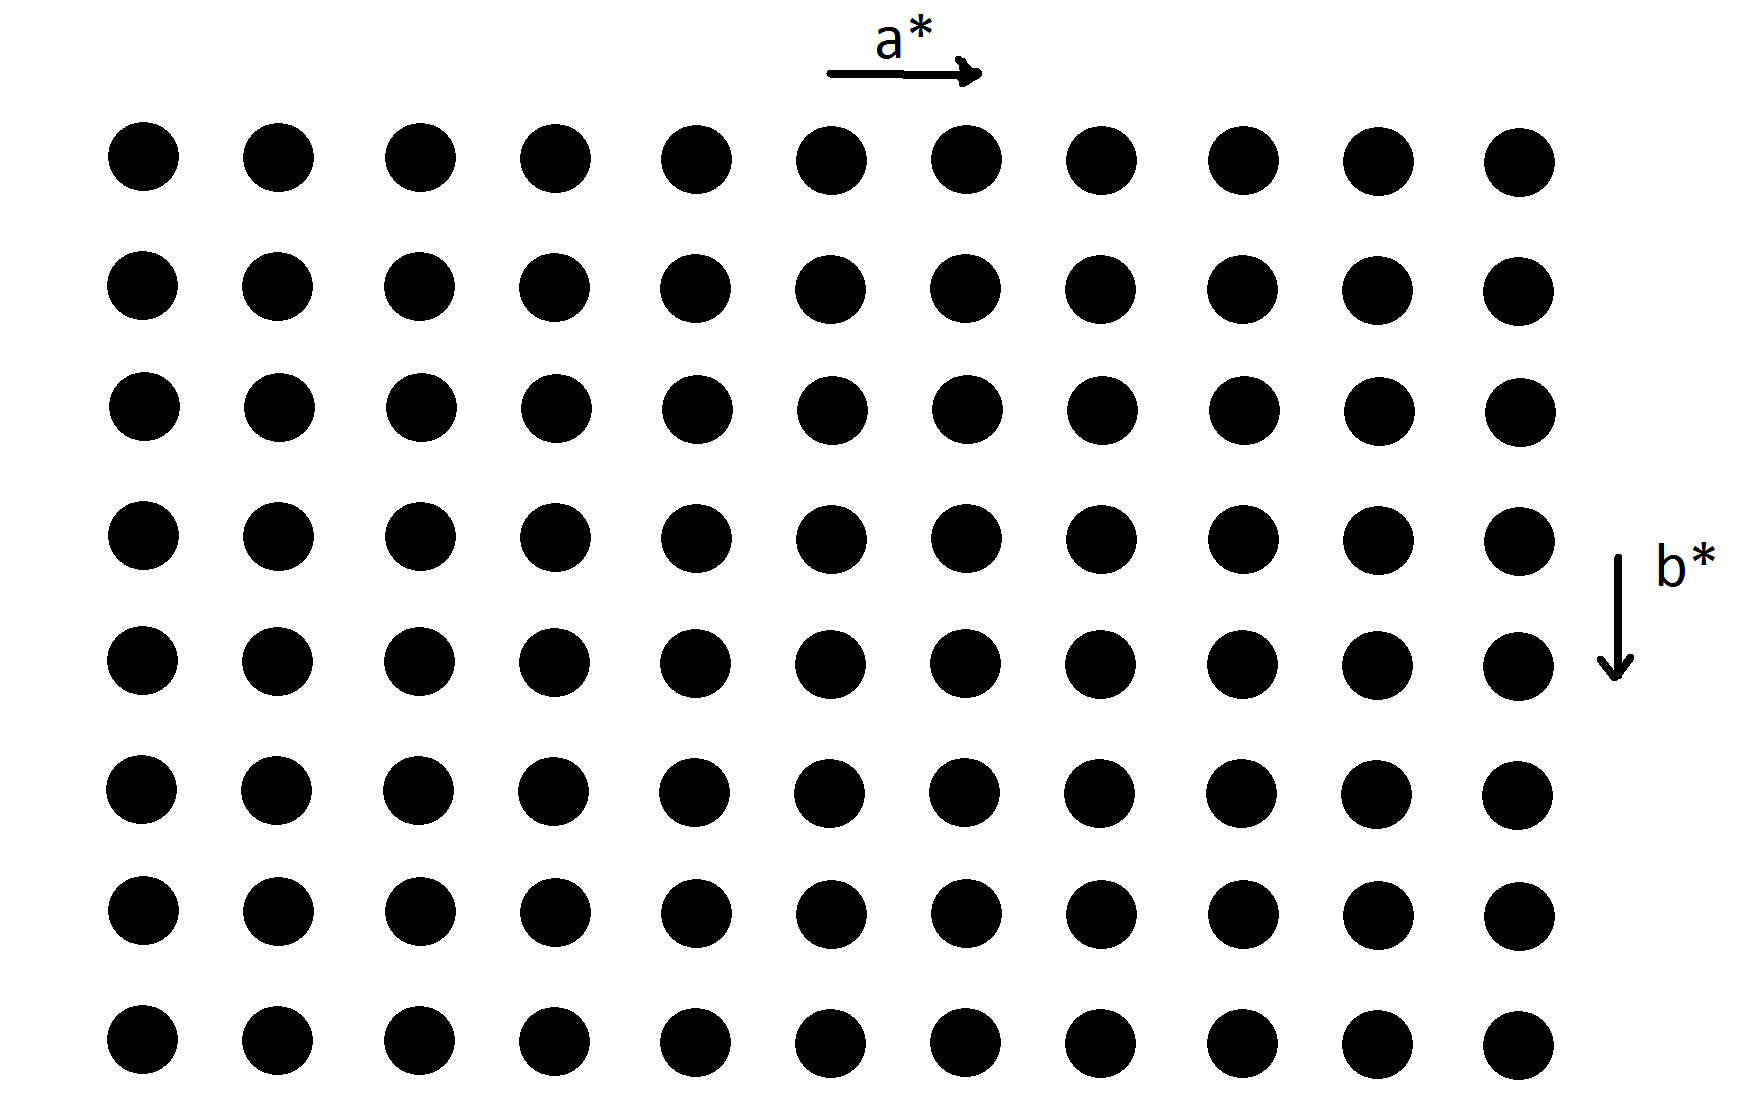
\includegraphics[scale=0.22]{1.png}
		\caption{ Red de puntos.}
\end{figure}


\vspace{\baselineskip}
En esta red de puntos elegimos un destino al que llegará nuestro haz incidente y determinamos los vectores de red reciproca como a$\ast$  y b$\ast$  como se indica en la figura 2. 


\begin{figure}[H]
	\centering
		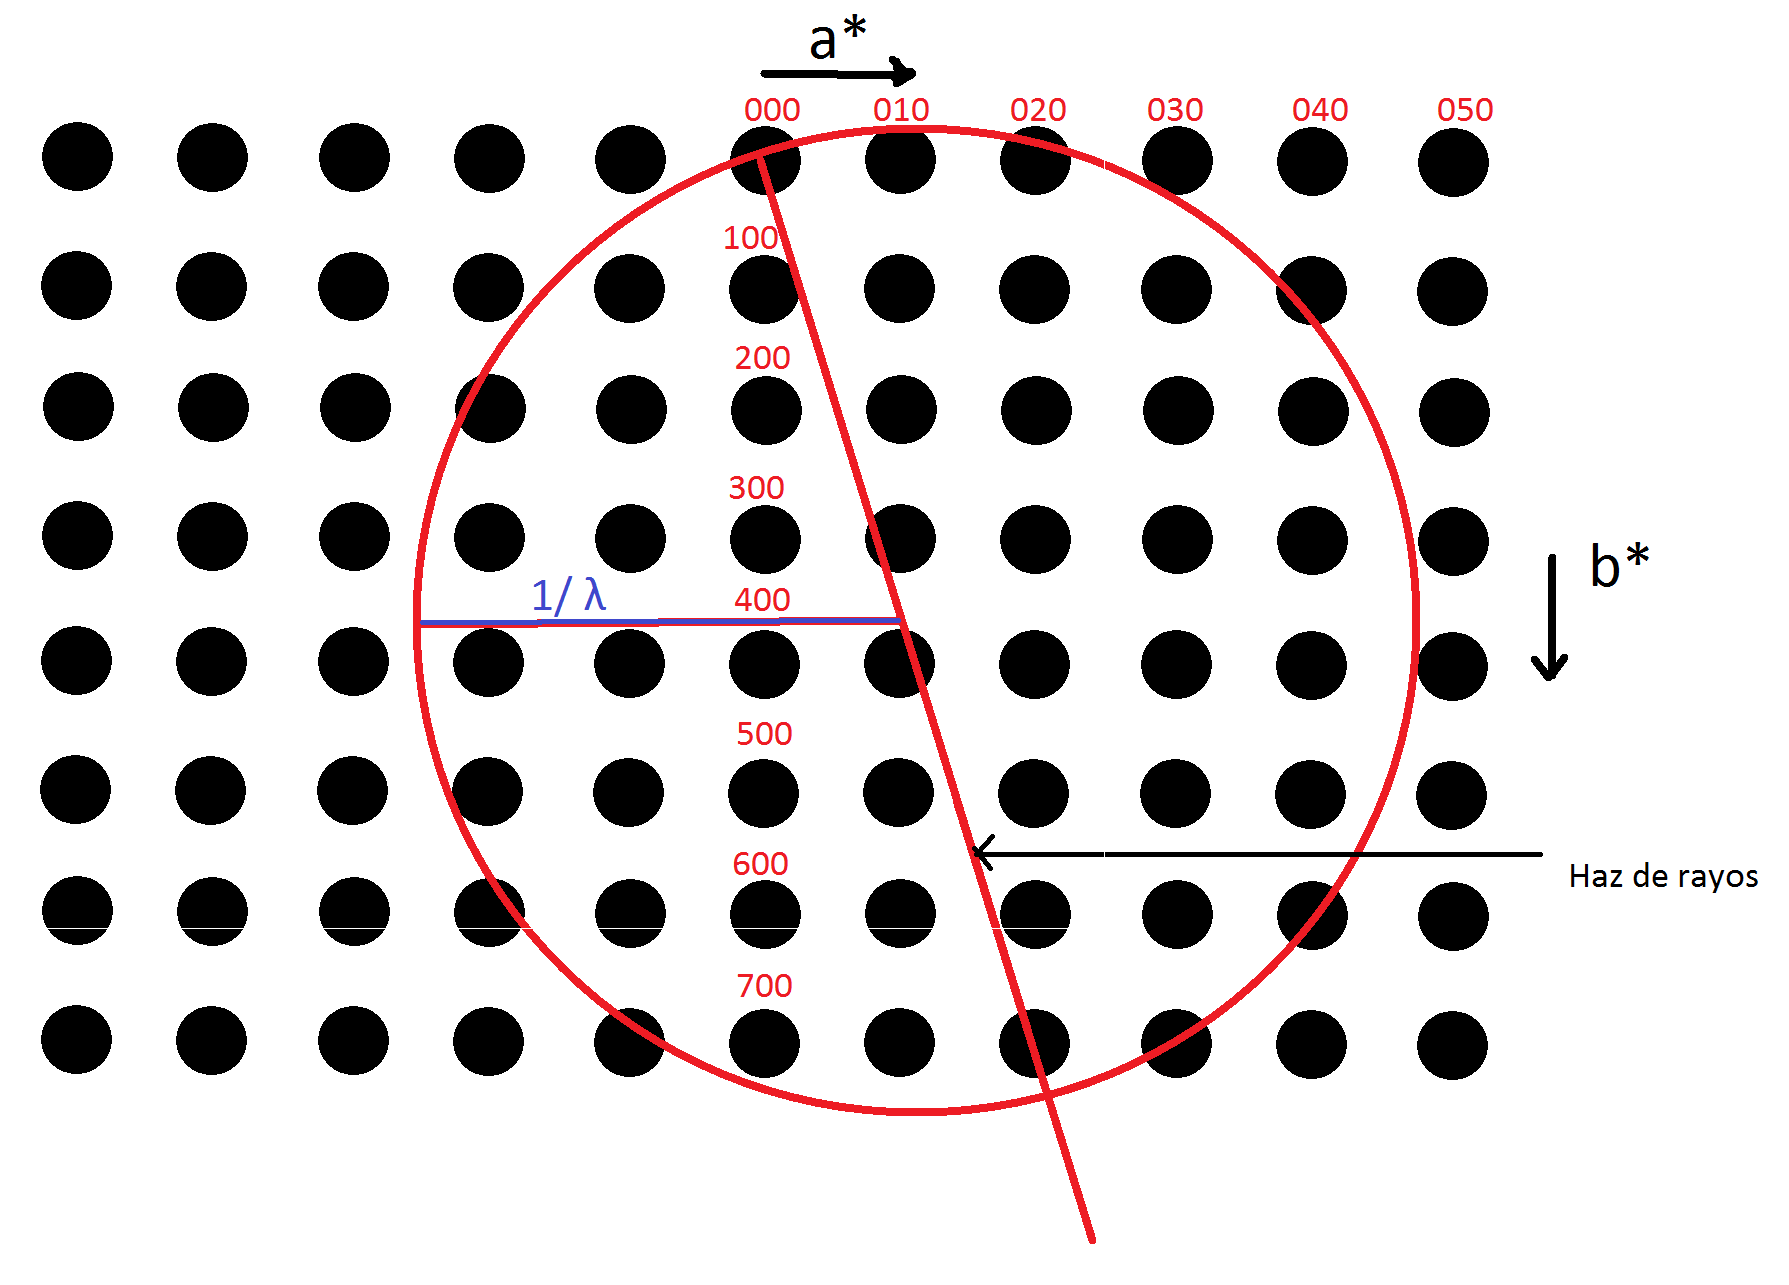
\includegraphics[scale=0.22]{2.png}
	\caption{Construcción de esfera de Edwald}
\end{figure}


Ahora si se cambia la dirección del haz de rayos X, se puede observar que en la superficie interna de la esfera aparece lo que parece el fenómeno de la reflexión.


\begin{figure}[H]
	\centering
		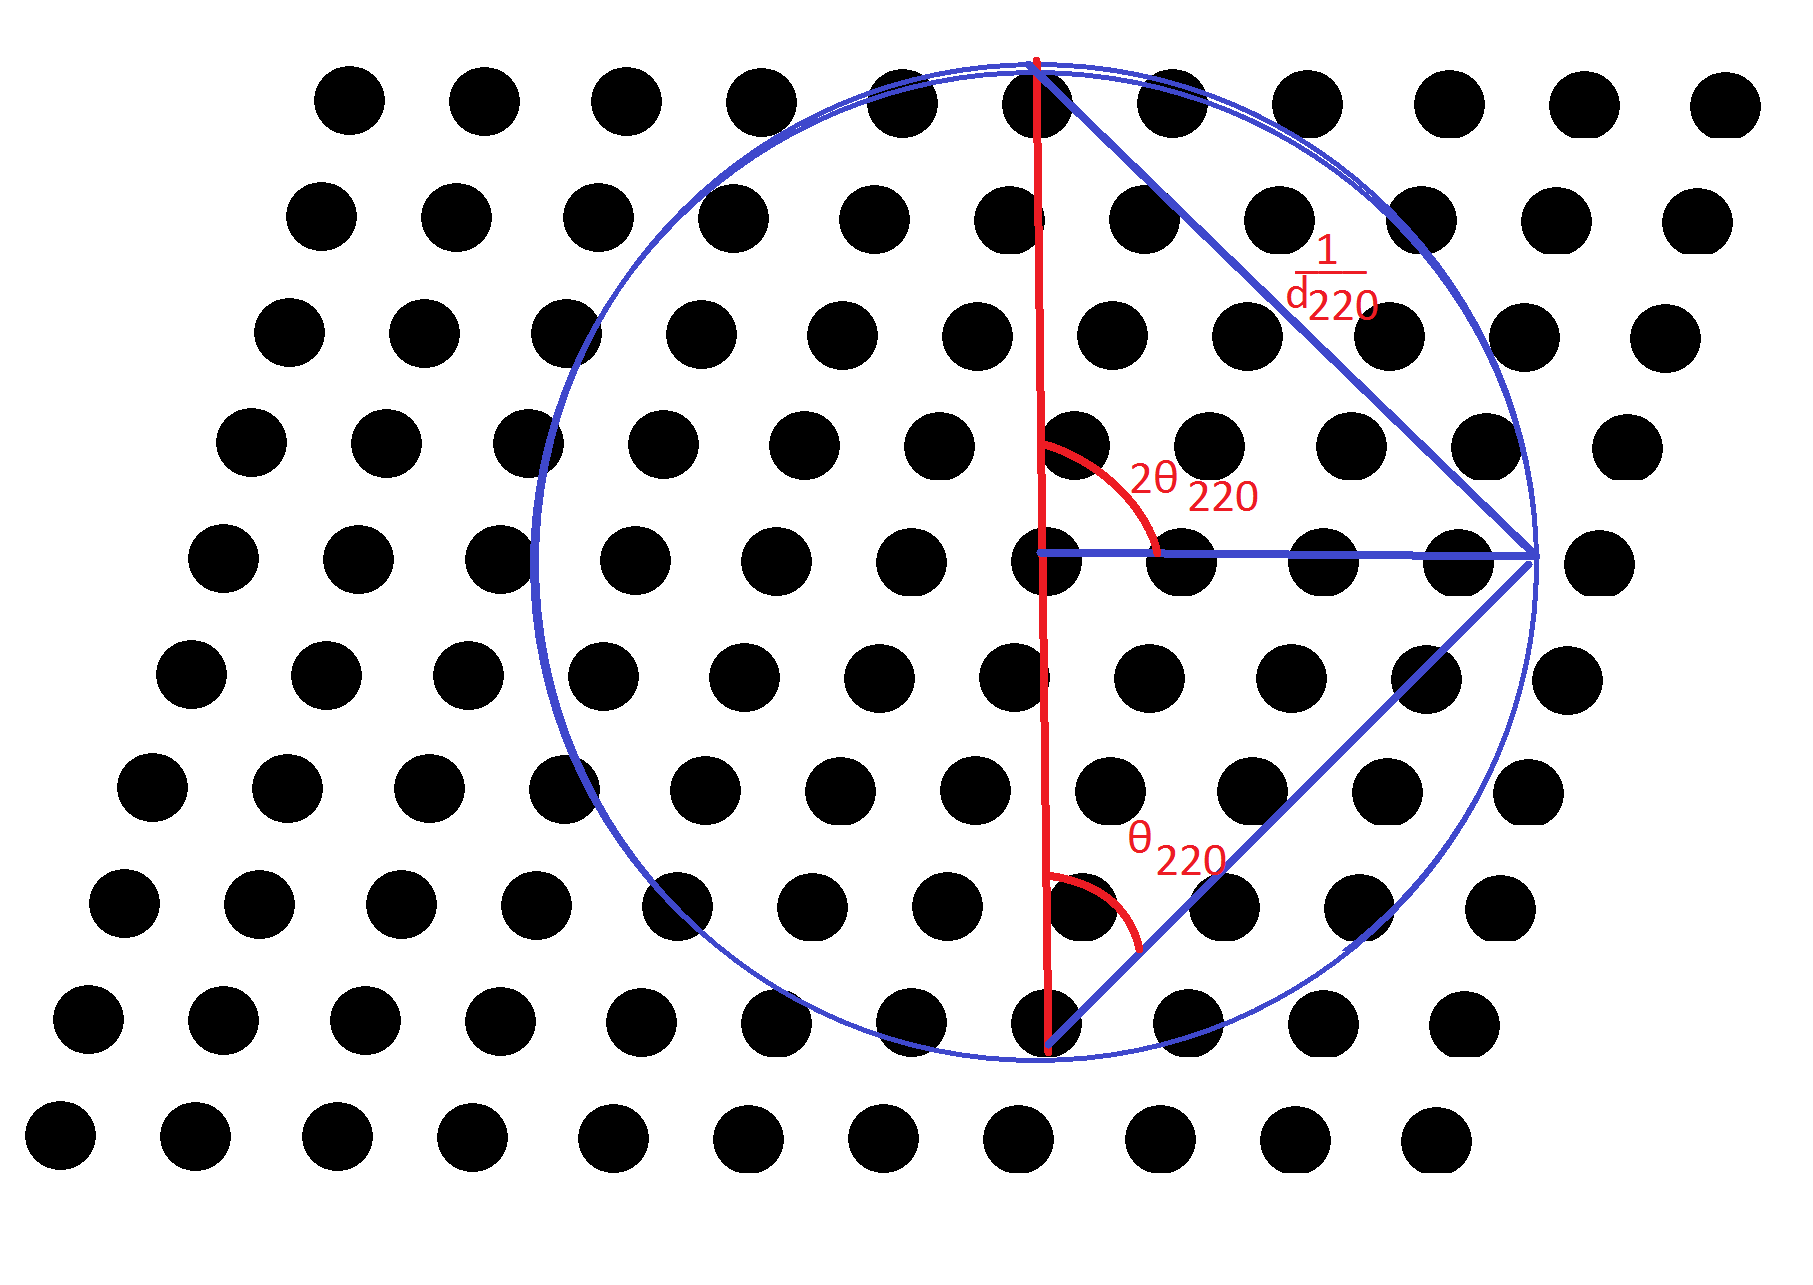
\includegraphics[scale=0.18]{3.png}
    \caption{Esfera de Edwald}
\end{figure}


\section{¿ Que son los índices de Miller, Por qué se conocen así?}

Los índices de Miller fueron presentados por propuestos por William Hallowes Miller en 1839. Los índices de Miller (h, k, l), en la cristalografía se definen como los recíprocos de las intercepciones donde el plano cristalográfico corta los ejes (x, y, z).

\subsection{Ejemplo 1}
Una forma simple de ilustrar un plano es la siguiente. Si tenemos un cubo de dimensiones (1x1x1) ubicado en el origen.

\begin{figure}[H]
	\centering
		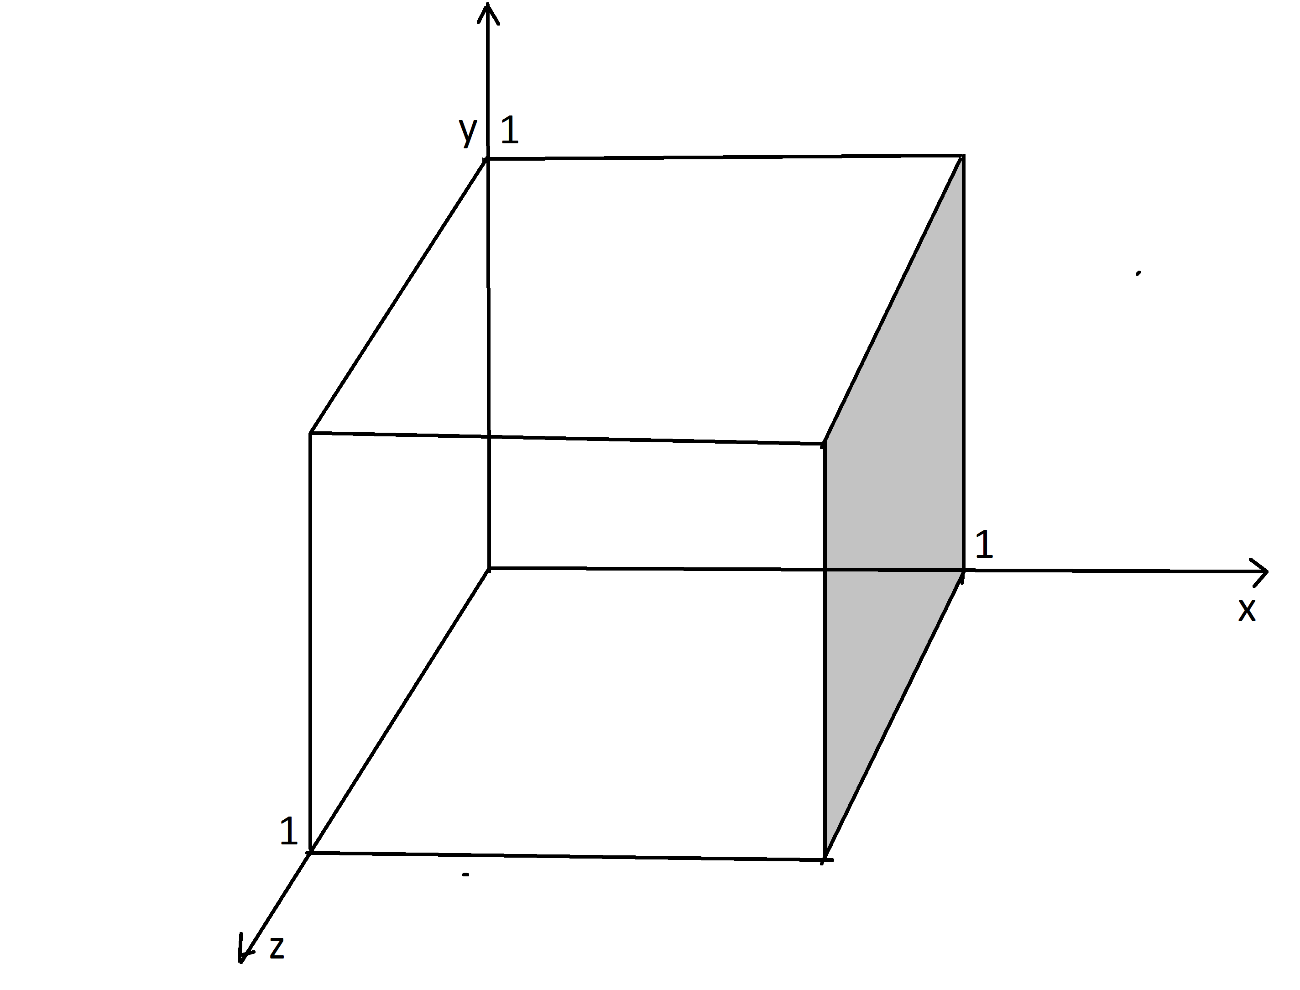
\includegraphics[scale=0.5]{4.png}
		\caption{cubo de arista 1}
\end{figure}


En este cubo podemos observar que se ha rellenado la cara que da hacía el eje x. Esto significa que tenemos un plano cristalográfico con índices de Miller (1, 0, 0).Donde para verificar, observamos que las intercepciones en los ejes son:

\begin{align*}
    Eje x = 1 \\
    Eje y = \infty \\
    Eje z = \infty \\
\end{align*}
    
De esta forma, los índices de Miller para este ejemplo son.:

\begin{equation*}
    \left( \frac{1}{1},\frac{1}{\infty},\frac{1}{\infty} \right) =  (1, 0, 0)
\end{equation*}

\subsection{Ejemplo 2}
Para ver con más detalles los índices de Miller y su aplicación en la cristalografía. Se encontrará el plano cristalográfico correspondiente a  (1, 2, 2).

Como se necesita encontrar los puntos de cortes en cada eje, se buscará que los valores en 1, 2, 2 estén dentro del cubo para determinar los cortes. Para esto dividiremos cada valor entre dos. 

\begin{equation*}
(1/2, 2/2, 2/2) = (1/2, 1, 1)
\end{equation*}

Si buscamos los puntos de corte, podemos encontrar el plano cristalográfico correspondiente a (1, 2, 2)

\begin{figure}[H]
	\centering
		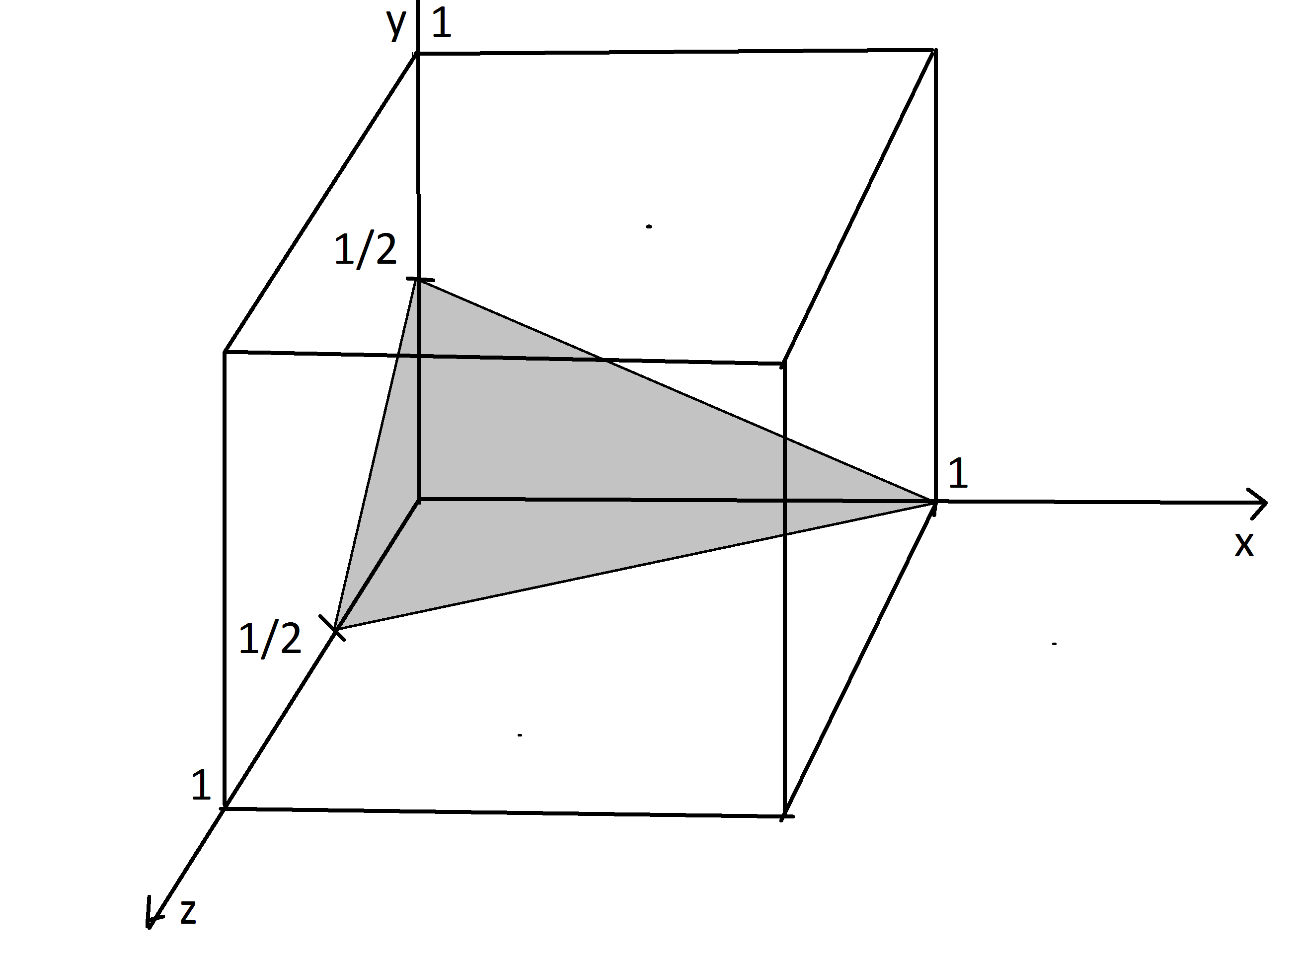
\includegraphics[scale=0.5]{5.png}
	\caption{plano cristalografico (2,1,1)}
\end{figure}


\vspace{\baselineskip}
En esta representación se puede identificar que el eje x se corta en 1, el eje y se corta en 1/2 y el eje z se corta en 1/2. 

\section{Haga un cuadro de las estructuras cristalinas que existen}

La materia en estado solido puede encontrarse en diferentes estados dependiendo de las escalas sobre las que presente orden en sus componentes, estas son : 

\begin{itemize}
    \item sin orden:  gases monoatómicos 
    \item orden de corto alcance:  materiales amorfos  
    \item orden de largo alcance:  materiales cristalinos (mono, poli)
    \item cristales liquidos: orden de corto alcance y de largo alcance en pequeños volumenes.
\end{itemize}

 \begin{figure}[H]
     \centering
     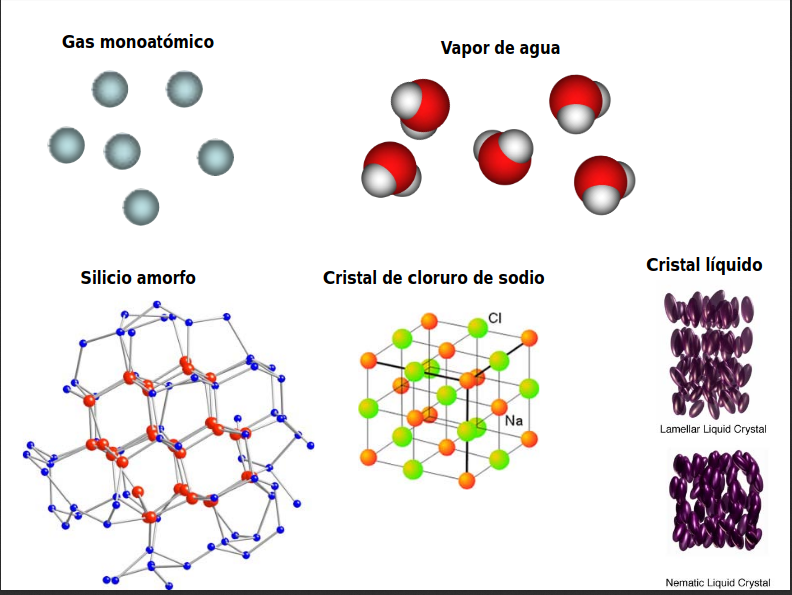
\includegraphics[scale=0.35]{Q3.png}
     \caption{ orden en las diferentes escalas del estado solido}
     \label{fig:my_label}
 \end{figure}


Dos sistemas importantes a estudiar son los de corto y largo alcance, amorfos y cristalinos.

\subsection{Materiales Amorfos} 
Son aquellos en los cuales el orden de sus estructuras no cumplen periodicidad espacial.

Como los átomos no están dispuestos en sus posiciones de equilibrio la tendencia natural es cristalizar, eso conduce a una mayor estabilidad termodinámica.
Ejemplos de estos son los vidrios y geles.


\subsection{Materiales Cristalinos}

Un cristal ideal es la repetición infinita de unidades idénticas en el espacio. La estructura de todos los cristales puede definirse en términos de una red, un arreglo de puntos en el espacio, en donde cada átomo ocupa un punto de dicha red.En este contexto se debe hacer distinción entre:

\begin{center}
Grupo de átomos - BASE \\
Arreglo periódico de puntos en el espacio  - RED
\end{center}

La red se define por un grupo de 3 vectores fundamentales o primitivos 

\begin{equation*}
    \bf{T} = a_{1} \bf{u_1} + a_{2}\bf{u_2} + a_{3}\bf{u_3}   
\end{equation*}


Existen múltiples formas de elegir dichos vectores, lo importante y conveniente es saber elegirlos puesto estos definirán la celda primitiva o unitaria. Una celda primitiva es la celda con el mínimo volumen que al repetirse llena completamente el espacio. En esta solo hay un punto de red.

\subsection{Tipos especiales de redes}

Estas comparten ciertas características que nos permiten clasificarlas, es decir, obedecen cierta simetría.En estas los vectores \textbf{$a_{i}$} deben cumplir restricciones tal que cumplan con la inerrancia bajo operaciones de simetría. Estas redes especiales se conocen como REDES DE BRAVAIS.

El número de redes de bravais que existen según las dimensiones de la red es finito, siendo 5 para redes 2D y 14 para las redes 3D. A continuación se mostraran cada una de estas: 

 \begin{figure}[H]
    \centering
	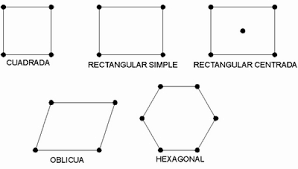
\includegraphics[width=0.8\linewidth]{Q.png}
	\caption{estructuras cristalinas en 2D}
\end{figure}

\begin{figure}[H] 
    \centering
    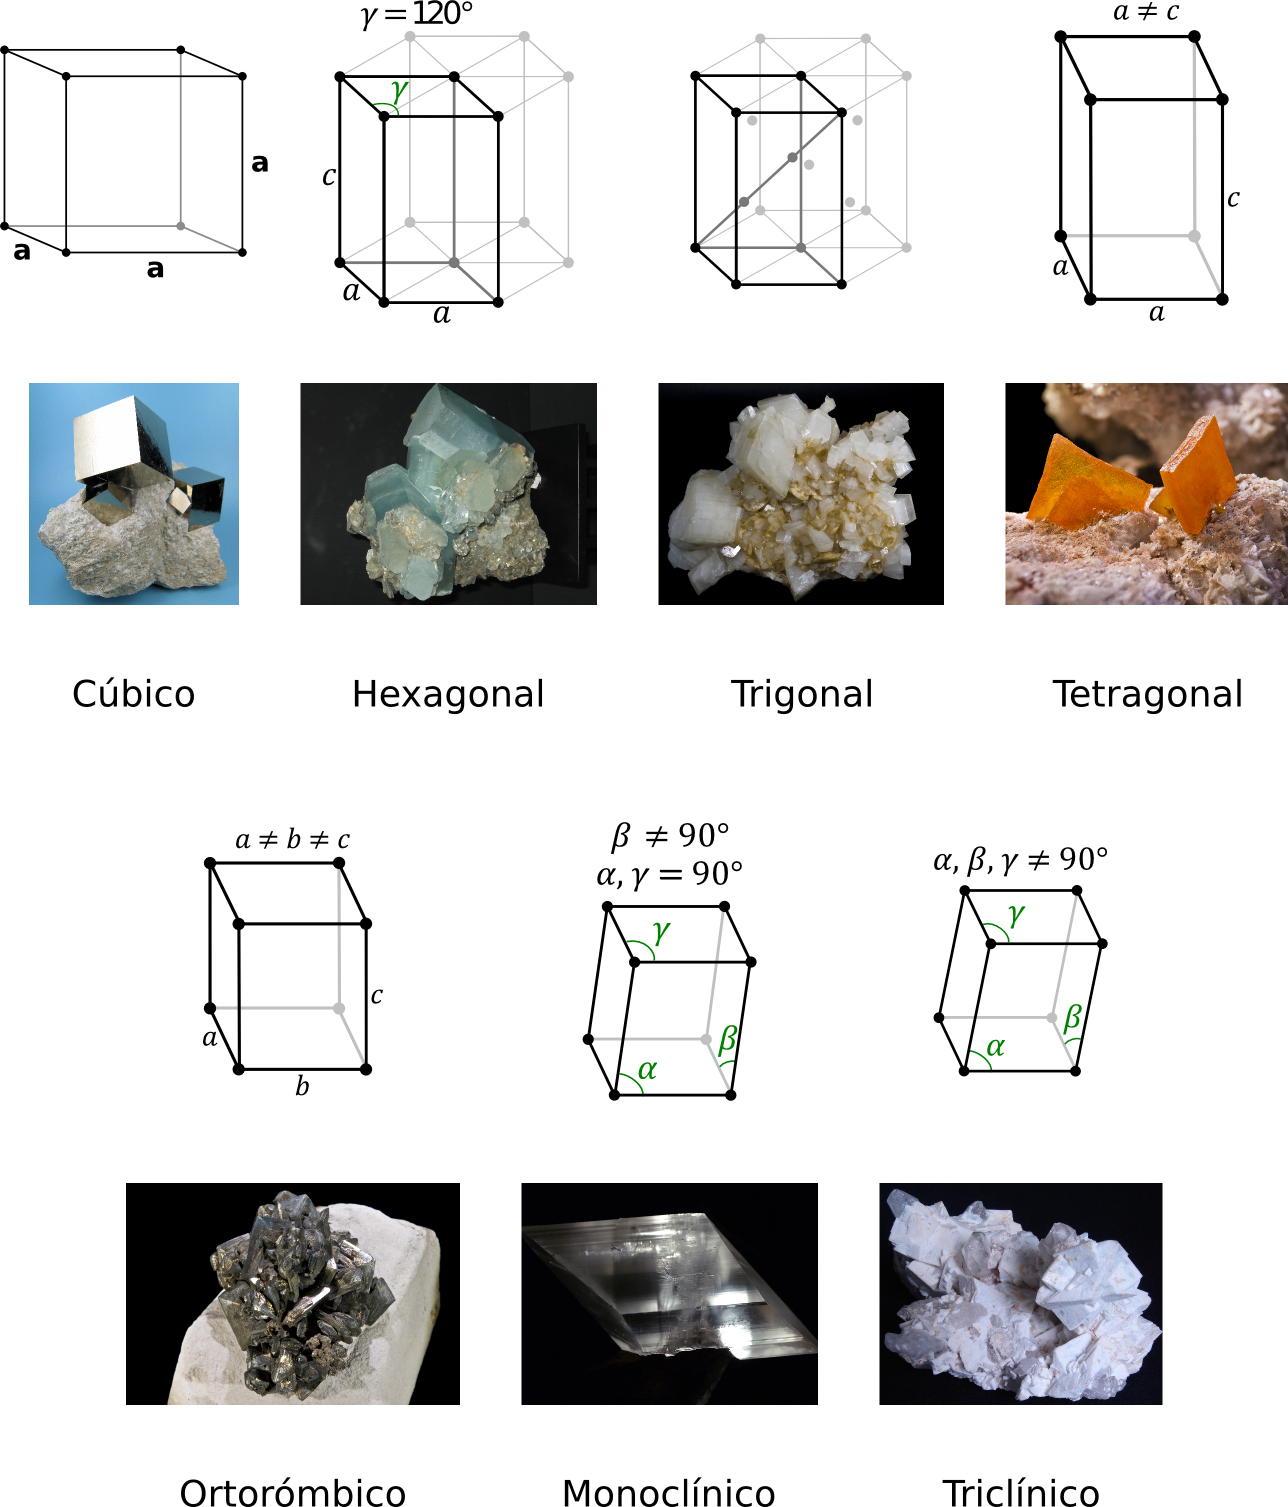
\includegraphics[scale= 0.2]{i.png}
    \caption{Estructuras cristalinas en 3D}
\end{figure}


\section{Dibuje la estructura cristalina de la escapolita e identifique sus propiedades}

Hace parte del grupo de materiales Tectosilicatos que forman una serie de solución solida entre dos extremos. Meionita de calcio. Merialita con sodio.Se encuentran sus cristales en pegmatitas (Rocas metamorficas), se caracteriza por presentar varios colores : incoloro, rosa, purpura, azul, amarilla, gris,café.

 \begin{figure}[H]
    \centering
	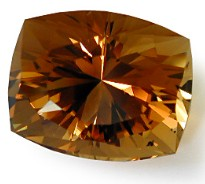
\includegraphics[width=0.3\linewidth]{k.jpg}
	 \caption{escapolita en pegmatita}
\end{figure}

\begin{table}[]
    \centering
    \begin{tabular}{|c|c|}
    \hline
      Gemología 	&   Material : escapolita	\\
      \hline
        Especie: painita 	& Composición  :	Na4Al3Si9O24Cl - Ca4Al6Si6O24(CO3,SO4)\\
        clase: zilicatos	& Sistema cristalino : Tetragonal 	\\
        grupo: Tectosilicatos	& Hábito  cristalino: Prisma con caras irregulares	\\
        color: variados palidos	&		\\
        brillo: vítreo	&		\\
    \hline
    \end{tabular}
    \caption{Caracteristicas principales de la escapolita}
    \label{tab:my_label}
\end{table}


\subsection{Propiedades}
 Las proiedades físicas de la escapolita se presentan a continuación: 
 
\begin{table}[H]
    \centering
    \begin{tabular}{|c|c|}
        \hline
        Propiedad & \\
        \hline
         Color &	Marrón, marrón anaranjado\\
        Índice refraccion &	1,540 - 1,577 \\
        Birrefringencia	& 0,009 - 0,037 \\
        Signo Óptico &	(-) \\
        Dureza (Mohs) &	5,5 - 6 \\
        Exfoliación	& Fácil \\
        Peso esp. &	2,60 - 2,70 \\
        Espectro absorción &El espectro de absorción presenta dos líneas significativas a 652 y 663 nm \\ 
        \hline
    \end{tabular}
    \caption{Propiedades física de la escapolita}
    \label{tab:my_label}
\end{table}


 \begin{figure}[H]
    \centering
	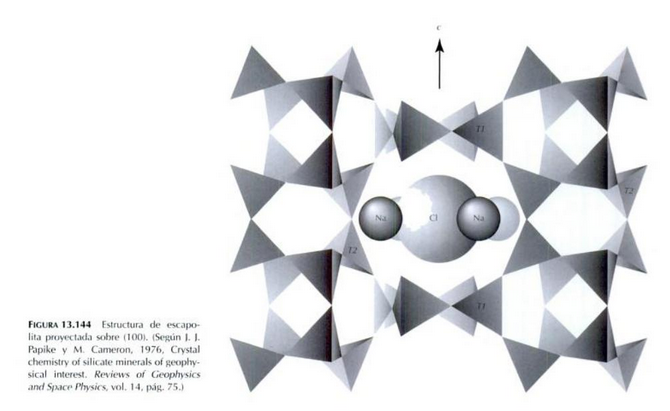
\includegraphics[scale= 0.7]{g.png}
	\caption{Estructura de la escapolita}
\end{figure}



La estructura de la escapolita (Figura 10 )consta de una armazón de tetraedros de  SiO4 y AlO4 con grandes cavidades que contienen iones  (Ca,Na) y grupos aniónicos(CO3, Cl2, SO4) y grupos aniónicos (CO3, Cl2,SO4).\\
\textbf{Yacimientos:}	Canadá, Mozambique, Tanzania, Birmania y Kenia.\\
\textbf{Observaciones:}	La escapolita se encuentra comprendida en la serie isomórfica de la marialita por un extremo y por el otro la meionita. Por tanto, como su fórmula química varía ligeramente podemos esperar ligeras variaciones en sus constantes físicas. Hay escapolita ojo de gato. Muestra fluorescencia fuerte de color naranja con luz ultravioleta de onda larga. Debemos tener cuidado con esta gema porque se exfolia fácilmente.


\newpage

\section*{Bibliografia}

\begin{enumerate}
    \item Solid State Physics. Ashcroft Mermin\\

    \item Introducción a la física del estado sólido.  Charles Kittel.\\

    \item BLOQUE II.- ESTRUCTURATema 2.- Estructura de la Materia* James F. Shackerlford“Introducción   a   la   Ciencia   de   Materiales   para   Ingenieros”. Cuarta edición. Ed. Prentice Hall (1998)* Pat L. Mangonon“Ciencia de Materiales: Selección y Diseño” Ed. Pearson Educación( 2001)\\

    \item estructura cristalina de solidos.Introducción a la •Ciencia de Materiales•M. Bizarro\\

    \item manual de mineralogía, Volumen 2. Escrito por Cornelis Klein, Cornelius S. Hurlbut pag.608\\

\end{enumerate}

\end{document}

